\begin{problem}
Copie el programa~\ref{code:elliptic3D.m} y modifique lo siguiente:

\begin{enumerate}
      \item

            ¿Cuál es el dominio de la EDP (la región donde la PDE se cumple)?

            \begin{solution}
                  El dominio de la EDP es
                  \begin{math}
                        \Omega=
                        \left[
                              0,7
                              \right]\times
                        \left[
                              0,8
                              \right]\times
                        \left[
                              0,9
                              \right]
                  \end{math}
            \end{solution}

      \item

            ¿Cuál es la ecuación que resuelve este ejemplo?

            \begin{solution}
                  La ecuación que resuelve es la ecuación de Laplace.
            \end{solution}

      \item

            ¿Cuál es la función de fuerza o el lado derecho?

            \begin{solution}
                  Es cero.
            \end{solution}

      \item

            ¿Qué tipo de condiciones de contorno?

            \begin{solution}
                  Se tiene condiciones Dirichlet.
            \end{solution}

      \item

            Cambie la condición de contorno a 100 en la cara frontal y posterior del cubo.

            \begin{solution}
            \end{solution}

      \item

            Ejecute el ejemplo con todos los cambios que ha realizado.

            \begin{solution}
            \end{solution}
\end{enumerate}
\end{problem}

\begin{listing}[ht!]
      \tiny
      \centering
      \inputminted[frame=single,framesep=10pt,linenos,firstline=1,lastline=38,highlightlines={14,15}]{octave}{../examples/octave/elliptic3D.m}
      \caption{Programa~\texttt{elliptic3D.m}}
      \label{code:elliptic3D.m}
\end{listing}

\begin{figure}[ht!]
      \centering
      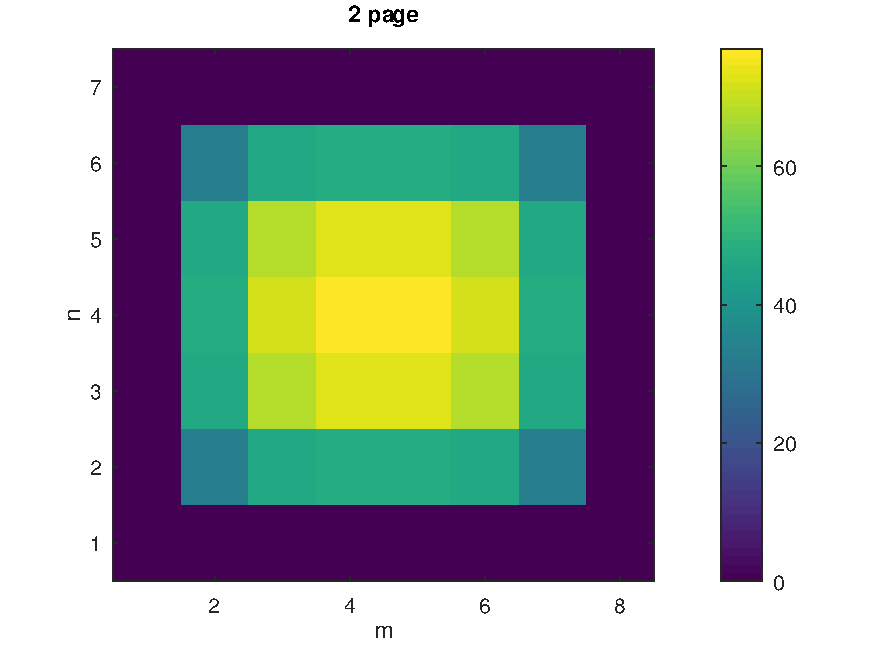
\includegraphics[width=.6\paperwidth]{../examples/octave/elliptic3D.pdf}
      % \caption{Solución al problema usando \mintinline{octave}|k=6| y \mintinline{octave}|m=2k+1=13|.}
\end{figure}